\section{Introduction}\label{sec:intro}

Nowhere dense classes of graphs were introduced 
by Ne\v set\v ril and Ossona de 
Mendez~\cite{nevsetvril2010first,nevsetvril2011nowhere} as a 
general and abstract model
capturing uniform sparseness of graphs. These classes generalize many 
familiar classes of sparse graphs, such as planar graphs, graphs 
of bounded treewidth,  graphs of bounded degree, and, in fact, 
all classes that exclude a fixed 
topological minor.
Formally, a class $\CCC$ of graphs is {\em{nowhere dense}} if there is a function $t\colon \N\to \N$ such that for every $r\in \N$, 
no graph~$G$ in~$\CCC$ contains the clique $K_{t(r)}$ on $t(r)$ vertices  as  {\em{depth-$r$ minor}},
i.e., as a subgraph of a graph obtained from $G$ by contracting mutually disjoint  subgraphs of radius at most~$r$ to single vertices.
The more restricted notion of {\em{bounded expansion}} requires in addition that for every fixed $r$, there is a constant (depending on $r$) upper bound on the ratio 
between the number of edges and the number of vertices in depth-$r$ minors of graphs from $\CCC$.

The concept of nowhere denseness
turns out to be very robust, as witnessed by the fact that 
it admits multiple different characterizations, uncovering intricate connections to seemingly distant branches of mathematics.
For instance,  nowhere dense graph classes can be characterized 
by upper bounds on the density of bounded-depth (topological) 
minors~\cite{nevsetvril2010first,nevsetvril2011nowhere},
by uniform quasi-wideness~\cite{nevsetvril2011nowhere} (a notion introduced by
Dawar~\cite{dawar2010homomorphism} in the context of homomorphism
preservation properties), by low tree-depth
colorings~\cite{nevsetvril2008grad}, by generalized coloring
numbers~\cite{zhu2009coloring}, by sparse neighborhood
covers~\cite{GroheKRSS15,grohe2014deciding}, by a game called the
splitter game~\cite{grohe2014deciding}, and by the model-theoretic
concepts of stability and independence~\cite{adler2014interpreting}.
For a broader discussion on graph theoretic sparsity we refer to the book
of Ne\v{s}et\v{r}il and Ossona de Mendez~\cite{sparsity}.

The combination of combinatorial and logical methods yields a powerful toolbox for the study
of nowhere dense graph classes. In particular, 
the result of Grohe, Kreutzer and the second author~\cite{grohe2014deciding} exploits 
this combination in order to prove that  a given
first order sentence $\varphi$ can be evaluated in time 
$f(\varphi)\cdot n^{1+\epsilon}$ on $n$-vertex graphs from a fixed nowhere dense class of graphs $\CCC$, for any fixed real $\epsilon>0$ and some function $f$.
On the other hand, provided $\CCC$ is closed under taking subgraphs, it is known that if $\CCC$ is not nowhere dense,
then there is no algorithm with running time of the form $f(\varphi)\cdot n^c$ for any constant~$c$ under plausible complexity assumptions~\cite{dvovrak2013testing}.
In the terminology of parameterized complexity, these results show that the notion of nowhere denseness exactly characterizes subgraph-closed classes where model-checking first order logic
is fixed-parameter tractable, and conclude a long line of research concerning the parameterized complexity of the model checking problem for sparse graph classes (see \cite{grokre11} for a survey). 


\paragraph{Summary of contribution.} In this paper, we continue the study of the 
interplay of combinatorial and logical properties
of nowhere dense graph classes, and provide
new upper bounds on several
quantities appearing in their logical study.
Our main focus is on the notion of \emph{VC-density} for first order formulas. This concept originates from model theory and 
aims to measure the complexity of set systems definable by first order formulas, similarly to the better-known VC-dimension.
We give optimal bounds on the VC-density in nowhere dense graph classes, and in particular we show that these bounds are ``as good as one could hope for''.

We also provide new upper bounds on quantities related to {\em{stability}} and {\em{uniform quasi-wideness}} of nowhere dense classes.
For stability, we provide explicit and computable upper bounds on the \emph{ladder index} of any first order formula on a given nowhere dense class.
For uniform quasi-wideness, we give a new, purely combinatorial proof of polynomial upper bounds on {\em{margins}}, that is, functions governing this notion.
We remark that the existence of upper bounds as above is known~\cite{adler2014interpreting,siebertz2016polynomial}, but the proofs are based on nonconstructive arguments, 
notably the compactness theorem for first order logic. Therefore, the upper bounds are given purely existentially and are not effectively computable.
Contrary to these, our proofs are entirely combinatorial and effective, yielding computable upper bounds.

We now discuss the relevant background from logic and model theory, in order to motivate and state our results.



\paragraph{Model theory.}Our work is inspired by ideas from model theory,  more specifically, from \emph{stability theory}.
  The goal of {stability theory}
  is to draw certain dividing lines
  specifying abstract properties of 
  logical structures which allow the development 
  of a good structure theory. There are many such dividing lines, depending on the specifics of the desired theory. One such dividing line encloses the class of \emph{stable structures}, 
  another encloses the larger class of \emph{dependent structures} (also called \emph{NIP}). 
  A general theme is that the existence of a manageable structure is strongly related to
  the non-existence of certain forbidden patterns on one hand,
and on the other hand, to bounds on cardinalities
of certain \emph{type sets}.  
  Let us illustrate this phenomenon more concretely.

For a first order formula 
$\phi(\tup{x},\tup{y})$ 
 with free variables
split into  $\tup{x}$ and $\tup{y}$,
a \emph{$\phi$-ladder}
of length $n$ in a logical structure $\str A$ is a sequence $\tup{u}_1,\ldots, \tup{u}_{n},
\tup{v}_1,\ldots, \tup{v}_{n}$ of tuples of elements of~$\str A$ 
such that 
\[\strA\models\phi(\tup{u}_i,\tup{v}_j)\ \Longleftrightarrow\ i\leq j\qquad \text {for all $1\leq i,j\le n$.}\]

The least  $n$ for which 
there is no $\phi$-ladder of length $n$ is 
the \emph{ladder index} 
of $\phi(\tup{x},\tup{y})$ in~$\str A$ (which may depend on the split of the
variables, and may be $\infty$ for some infinite structures $\str A$). A class of structures $\CCC$ is \emph{stable} if
the ladder index of every first order formula $\phi(\tup{x},\tup{y})$ over
structures from~$\CCC$ is bounded by a constant depending only on $\phi$ 
and~$\CCC$. This notion can be applied to a single infinite structure $\str A$, by considering the class consisting of $\str A$ only.
Examples of stable structures include $(\str N,=)$,
the field of complex numbers $(\str C,+,\times,0,1)$,
as well as any vector space $V$ over the field of rationals, treated as a group with addition. On the other hand, $(\str Q,\le)$ and the field of reals $(\str R,+,\times,0,1)$ are not stable,
as they admit a linear ordering which is definable by a first order formula.
Stable structures turn out to have more graspable  structure than unstable ones, as they can be equipped with various notions 
useful for their study, such as
\emph{forking independence} (generalizing linear independence in vector spaces)
and \emph{rank} (generalizing dimension).
We refer to the textbooks~\cite{pillay,tent2012course} for an introduction to stability theory.

  One of concepts studied in the early 
  years of stability theory is 
  a property of infinite graphs  called \emph{superflatness}, introduced by Podewski and Ziegler~\cite{podewski1978stable}.
  The definition of superflatness is the same as   of nowhere denseness, but 
   Podewski and Ziegler,
  instead of applying it to an infinite class of finite graphs, apply it to a single infinite graph.
  The main result of~\cite{podewski1978stable} is that every superflat graph is stable.   
As observed by Adler and Adler~\cite{adler2014interpreting}, 
this directly implies  the following:
 \begin{theorem}[\cite{adler2014interpreting,podewski1978stable}]\label{thm:adleradler}
 	Every nowhere dense class of graphs is stable. Conversely, any stable class of finite graphs which is subgraph-closed  is nowhere dense.
 \end{theorem}
 Thus, the notion of nowhere denseness (or superflatness) coincides with stability if we restrict attention to subgraph-closed graph classes.
 
The proof of Adler and Adler does not yield effective or computable upper bound on the 
ladder index of a given formula for a given nowhere dense class of graphs, as it relies on the result of Podewski and Ziegler, which in turn invokes compactness for first order logic.

\paragraph{Cardinality bounds.}
One of the key insights provided by the work of Shelah is that stable classes can be characterized by admitting strong upper bounds on the cardinality of \emph{Stone spaces}.
For a first order formula $\phi(\tup x,\tup y)$ 
with free variables partitioned into \emph{object variables} $\bar x$ and \emph{parameter variables} $\tup y$, a logical structure $\str A$,
and a subset of its domain $B$, define
the set of \emph{$\phi$-types} with parameters from~$B$, which are realized in~$\strA$, as follows\footnote{Here, $S^\phi(\str A/B)$ is the set  of types which are \emph{realized} in $\str A$. In model theory,
one usually works with the larger class of \emph{complete types}. This distinction will not be relevant here.}:
\begin{equation}\label{eq:stone-def}
\begin{split}
S^\phi (\strA/B) & = 
  \left\{\big\{\tup v\ \in B^{|\bar y|}\, \colon\, \strA\models\phi(\tup u,\tup v)\big\} \colon\, \tup u\in V(\strA)^{|\bar x|}\right\}\ \\ & \subset\  \Pow(B^{|\bar y|}).
 \end{split}
\end{equation}
Here, $V(\strA)$ denotes the domain of $\strA$ and $\Pow(X)$ denotes the powerset of $X$.
Putting the above definition in words, every tuple $\tup u\in V(\strA)^{|\bar x|}$ defines the set of those tuples $\tup v\in B^{|\bar y|}$ for which $\phi(\tup u,\tup v)$ holds.
The set $S^\phi(\strA/B)$ consists of all subsets of $B^{|\bar y|}$ that can be defined in this way.

Note that in principle, $S^\phi(\str A/B)$
may be equal to $\Pow(B^{|\bar x|})$, and therefore have very large cardinality compared to $B$, even for very simple formulas. 
The following characterization due to Shelah 
(cf. \cite[Theorem 2.2, Chapter II]{shelah1990classification})
shows that for stable classes this does not happen.
%\begin{theorem}%\label{thm:Shelah-stone-space}
A class of structures $\cal C$
	is stable if and only if 
	there is 
	an infinite cardinal $\kappa$
	such that the following holds for all
	structures
	$\str A$ in the elementary closure\footnote{The elementary closure of $\cal C$ is 
	the class of all structures $\str A$
	such that  every first order sentence $\phi$
	which holds in $\str A$ also holds in some $\str B\in \cal C$. Equivalently, it is the class of 
   models of the theory of $\cal C$.} of~$\cal C$, and 
   all $B\subset V(\str A)$:
\mbox{\textit{if} $|B|\le \kappa$, \textit{then} $
|S^\phi(\str A/B)|\le \kappa$.}
%\end{theorem}
Therefore,
Shelah's result provides an upper bound on the number of types, albeit using infinite cardinals, elementary limits, and infinite parameter sets.
 The cardinality bound provided by the above characterization %Theorem~\ref{thm:Shelah-stone-space},
 however, does not seem to  immediately translate to a result of finitary nature. As we describe below,
 this can be done using the notions of {\em{VC-dimension}} and {\em{VC-density}}.

\paragraph{VC-dimension and VC-density.} The notion of VC-di\-men\-sion was introduced by 
Vapnik and Chervonenkis~\cite{chervonenkis1971theory} 
as a measure of complexity of set systems, or equivalently of 
hypergraphs, and independently by Shelah~\cite{shelah1971stability} 
under the name of dependence (equivalence of the two notions
was observed by Laskowski~\cite{laskowski1992vapnik}).
%Over the years it
%has found important applications in many areas of
%statistics, discrete and computational geometry, 
%learning theory, and model theory. 

Formally, VC-dimension is defined as follows. 
Let $X$ be a set and let  $\FFF\subseteq \Pow(X)$ 
be a family of subsets of $X$.
A subset $A\subseteq X$ is \emph{shattered by $\FFF$} if
$\{A\cap F\colon F\in \FFF\}=\Pow(A)$; that is, every subset of $A$ can be obtained as the intersection of some set from $\FFF$ with $A$. 
The \emph{VC-dimension},
of $\FFF$ is the maximum size of a subset $A\subseteq X$ that is shattered by
$\FFF$.

%As observed by Laskowski~\cite{laskowski1992vapnik}, VC-dimension can be connected to concepts from stability theory introduced by Shelah.
For a given structure $\str A$, parameter set $B\subseteq V(\str A)$, and formula $\phi(\bar x,\bar y)$,
we may consider the family $S^\phi(\str A/B)$ of subsets of $B^{|\tup y|}$ defined using equation~\eqref{eq:stone-def}.
The \emph{VC-dimension} of $\phi(\bar x,\bar y)$ on $\str A$ is the VC-dimension of the family $S^\phi(\str A/V(\str A))$. 
In other words, the VC-dimension of $\phi(\bar x,\bar y)$
on $\str A$ is the largest cardinality of a finite
set $I$ for which there exist families of tuples $(\bar u_i)_{i\in I}$ and $(\bar v_J)_{J\subset I}$
of elements of $\str A$
such that  $$\strA\models\phi(\tup{u}_i,\tup{v}_J)\Longleftrightarrow i\in J\qquad \text {for all $i\in I$ and $J\subset I$.}$$
A formula $\phi(\bar x,\bar y)$ is \emph{dependent} on a class of structures $\cal C$
if there is a bound $d\in\N$ such that the VC-dimension of $\phi(\bar x,\bar y)$ on $\str A$ is at most $d$ for all $\str A\in\cal C$.
It is immediate from the definitions  that if a formula $\phi(\bar x,\bar y)$ is stable over $\cal C$, then it is also dependent on $\cal C$ (the bound being the ladder index). 
A class of structures  $\cal C$ is {\em{dependent}} if every formula $\phi(\bar x,\bar y)$ is dependent over $\cal C$. 
In particular, every stable class is dependent, and hence, by Theorem~\ref{thm:adleradler}, every nowhere dense class of graphs is dependent.
Examples of infinite dependent structures (treated as singleton classes) include 
$(\mathbb Q,\le )$ and the field of reals $(\mathbb R,\times,+,0,1)$. 

One of the main properties of VC-dimension is that it implies polynomial upper bounds on the number of different ``traces'' that a set system can have on a given parameter set.
This is made precise by the well-known Sauer-Shelah Lemma, stated as follows.
\begin{theorem}[Sauer-Shelah Lemma, \cite{chervonenkis1971theory,sauer1972density, shelah1972combinatorial}]\label{thm:sauer-shelah}
  For any family $\FFF$ of subsets of a set $X$, if the VC-dimension of $\FFF$ is $d$,
  then for every finite $A\subset X$,
\[|\setof{A\cap F}{F\in {\cal F}}|\le \sum_{i\geq 0}^d \binom{|A|}{i}\leq |A|^d+1.\] 
\end{theorem}
In particular, this implies that 
in a dependent class of structures $\cal C$, 
for every formula $\phi(\bar x,\bar y)$
there exists some constant $d\in \N$
such that
\begin{equation}\label{eq:nip}
|S^\phi(\str A/B)|\le |B|^d+1,	
\end{equation}
for all $\str A\in\cal C$ and finite $B\subset V(\str A)$.
%Unlike~Theorem~\ref{thm:Shelah-stone-space}, 
Unlike Shelah's characterization theorem of stable classes, this result 
is of finitary nature: it provides quantitative upper bounds on the number of different definable subsets of a given finite parameter set. 
Together with Theorem~\ref{thm:adleradler}, this implies that for every nowhere dense class of graphs %$\cal C$
and every first order formula $\phi(\bar x,\bar y)$,
there exists a constant \mbox{$d\in\N$} such that~\eqref{eq:nip} holds. 

For many structure classes $\cal C$ the combination of 
bounding VC-dimension and applying the
Sauer-Shelah Lemma yields a suboptimal upper bound of the form 
\eqref{eq:nip}. This 
motivates the notion of \emph{VC-density}, a notion closely related to 
VC-dimension. The \emph{VC-density} (also called the 
\emph{VC-exponent})
of a set system $\cal F$
on an infinite set $X$ is the infimum of all reals $\alpha>0$ such that 
$|\setof{A\cap F}{F\in \cal F}|\in \Oof(|A|^\alpha)$, for all finite $A\subset X$
(where the constants hidden in the $\Oof$ notation may depend on $\alpha$). 
Similarly, the VC-density of a formula $\phi(\bar x,\bar y)$ over a class of structures~$\cal C$
is the infimum of all reals $\alpha>0$
such that $|S^\phi(\str A/B)|\in \Oof(|B|^\alpha)$,
for all $\str A\in \cal C$ and all finite $B\subset V(\str A)$.
The Sauer-Shelah Lemma
implies that the VC-density (of a set system, or of a formula over a class of structures) is bounded from above by the VC-dimension. 
Our main result, Theorem \ref{thm:vc-density} below, provides optimal bounds on the VC-density in the setting of nowhere dense graph classes. In particular, we show that the VC-density of a formula $\phi(\bar x,\bar y)$ over a nowhere dense class $\cal C$ is bounded by $|\bar x|$.

\paragraph{Motivation.}
The motivation for finding bounds on the VC-density  comes from the fact that it is this quantity, rather than VC-di\-men\-sion, that is actually relevant in combinatorial
and algorithmic applications~\cite{Bronnimann1995,matouvsek1998geometric,Matousek:2004:BVI:1005787.1005789,chervonenkis1971theory,blumer1989learnability}. %, see also \autoref{sec:ep}.
Let us give an example from statistical learning theory. 
In the framework of \emph{probably approximately correct learning} 
(PAC learning, introduced by Valiant in~\cite{valiant1984theory}), a
learning algorithm receives a random sample $X$ of elements of a universe $\Omega$
and the restriction  $f|_X\from X\to\set{0,1}$
of an unknown function $f\from \Omega\to\set{0,1}$.
The goal is
to produce a function
$f'\from \Omega\to\set{0,1}$
from a certain class of possible 
functions $\cal C\subset 2^\Omega$,
called the \emph{concept class}, so that $f'$  coincides with $f$ on a set of inputs from $\Omega$
of large probability, for any fixed probability distribution on~$\Omega$.

More formally, 
 for a function $m(\epsilon,\delta)$, the concept 
class $\mathcal{C}$ is \emph{PAC-learnable} with sample size 
$m(\epsilon,\delta)$ if there is an algorithm,
such that for every $f\from \Omega\to\set{0,1}$, probability distribution on~$\Omega$, and numbers $\epsilon,\delta>0$,
the algorithm given  $\epsilon$ and $\delta$
and  the restriction of $f$ to a random sample $X\subset \Omega$ of size  $|X|\le m(\epsilon,\delta)$,
produces a function $f'\from \Omega\to \set{0,1}$, 
so that with probability at least $1-\delta$
(with respect to the random sample $X\subset \Omega$),  $\textrm{Pr}_{x\in\Omega}[f'(x)\neq f(x)]\le \epsilon$.

It is shown in \cite{chervonenkis1971theory,blumer1989learnability} 
that every concept class $\CCC$ is PAC-learnable with sample size
$m(\epsilon,\delta)=\max\left\{\frac{4}{\epsilon}\log \frac{2}{\delta},
\frac{8d}{\epsilon}\log \frac{13}{\epsilon}\right\}$, where $d$ is the
VC-dimension of the hypothesis space. 
The proof of this fact given in~\cite{blumer1989learnability} shows
that it suffices to choose the sample size $m=m(\epsilon, \delta)$ 
such that 
\mbox{$2\Phi(2m)\cdot
2^{-\epsilon m/2}\leq \delta$}, where $\Phi(2m)$ denotes the 
maximum number of distinct intersections of the concept class
with any subset of the instance space of size at most $2m$. 
Using the bounds of Theorem~\ref{thm:sauer-shelah} leads to
the above sample size $m(\epsilon,\delta)$. 

%TODO:write explicitly how this relates to VC-density. 


The following framework for learning in a logical setting was introduced
by Grohe and Tur\'an in~\cite{grohe2004learnability}. We assume
that the ground set of examples $A$ are elements, or more generally, 
tuples of elements, of a finite structure $\strA$, and concepts are 
first-order definable set systems exactly as defined in~(\ref{eq:stone-def}).
Grohe and Tur\'an proved that all definable set systems over classes 
of bounded local clique-width have bounded VC-dimension, and are hence
PAC learnable. Adler and Adler~\cite{adler2014interpreting} then observed
that over a subgraph closed class of structures, definable concepts are 
PAC-learnable if and only if the class is nowhere dense. Our improved
bounds on the number of types realized in a nowhere dense graph class, 
which we discuss next,
immediately lead to much smaller sampling sizes required for PAC learning 
first-order definable concepts on nowhere dense
graph classes. We note that~\cite{grohe2017learning,grohe2017learning2}
provide further advances in this framework, which are however orthogonal to ours.

In Theorem~\ref{thm:erdos-posa} below we give another example where bounds on the VC-density yield bounds on certain combinatorial quantities.
We refer to~\cite{aschenbrenner2016vapnik} for an overview of 
further applications of VC-dimension and VC-density in model
theory and to the surveys~\cite{furedi1991traces,matouvsek1998geometric} 
on uses of VC-density in
combinatorics. 

\paragraph{The main result.}
Our main result, Theorem~\ref{thm:vc-density} stated below, improves the bound~\eqref{eq:nip} for classes of sparse graphs
by providing essentially the optimum exponent.

% \newcounter{vcupper}
% \setcounter{vcupper}{\thetheorem}
 \begin{theorem}\label{thm:vc-density}
%\begin{restatable}{theorem}{vcupper}\label{thm:vc-density}
Let $\CCC$ be a nowhere dense class of graphs and let $\phi(\tup x,\tup y)$ be a first order formula
with free variables  partitioned  into object variables $\bar x$  and parameter variables $\bar y$. Let $\ell=|\bar x|$. Then 
for every $\epsilon>0$ 
there exists a constant~$c$ such that for every $G\in \CCC$ and every nonempty
$A\subseteq V(G)$, we have $|S^\phi(G/A)|\leq c\cdot |A|^{\ell+\epsilon}.$
%\end{restatable}
 \end{theorem}

In particular, Theorem~\ref{thm:vc-density} implies that
the VC-density of any fixed formula 
$\phi(\bar x,\bar y)$ over any nowhere dense class of graphs is $|\bar x|$, the number of object variables in $\phi$.

To see that the bounds provided by Theorem~\ref{thm:vc-density} cannot be improved, consider a formula $\phi(\bar x,y)$ (i.e. with one parameter variable) expressing that $y$ is equal to one of the entries of~$\bar x$. Then for each graph $G$ and parameter set $A$, $S^{\phi}(G/A)$ consists of all subsets of $A$ of size at most~$|\tup x|$, whose number is $\Theta(|A|^{|\tup x|})$. Note that
this lower bound applies to any infinite class of graphs, even edgeless ones.

We moreover show that, as long as we consider only subgraph-closed graph classes, the result of Theorem~\ref{thm:vc-density} also cannot be improved in terms of generality.
The following result is an easy corollary of known characterizations of obstructions to being nowhere dense.

% \newcounter{vclower}
% \setcounter{vclower}{\thetheorem}
   \begin{theorem}\label{thm:vc-density-lower-bound}
  %\begin{restatable}{theorem}{vclower}\label{thm:vc-density-lower-bound}
  Let $\CCC$ be a class of graphs which 
  is closed under taking subgraphs. 
   If $\CCC$ is not nowhere dense, then there is a formula 
  $\phi(x,y)$ such that for every $n\in \N$ there are $G\in\CCC$ and $A\subseteq V(G)$ 
  with $|A|=n$ and $|S^\phi(G/A)|=2^{|A|}$. 
  %\end{restatable}  
\end{theorem}

We prove in the appended full version of the paper that a similar
characterization theorem can be proved for bounded
expansion classes of graphs (all proofs that are omitted
in the conference version due 
to space constraints are marked with a $\star$ and can be 
found in the appendix). More precisely, we show that 
if $\CCC$ has bounded 
expansion, then there exists a constant~$c$ such that for every 
$G\in \CCC$ and every nonempty $A\subseteq V(G)$, we have 
$|S^\phi(G/A)|\leq c\cdot |A|^\ell$. Conversely, if $\CCC$ has 
unbounded expansion, then there is a formula $\phi(x,y)$ such 
that for every $c\in \mathbb{R}$ there exist $G\in\CCC$ and 
a nonempty $A\subseteq V(G)$ with $|S^\phi(G/A)|>c|A|$. 

\paragraph{Neighborhood complexity.}
To illustrate Theorem~\ref{thm:vc-density}, consider the case when
$G$ is a graph and  $\phi(x,y)$ is the formula with two variables $x$ and $y$ expressing that the distance between $x$ and $y$
is at most $r$, for some fixed integer $r$. In this case, $S^\phi(G/A)$ is the family consisting of all intersections $U\cap A$, for $U$ ranging over all balls of radius $r$ in $G$,
and  $|S^\phi(G/A)|$ is called the \emph{$r$-neighborhood complexity} of $A$.
The concept of $r$-neighborhood complexity in sparse graph classes has already been studied before.
In particular, it was proved by Reidl et al.~\cite{reidl2016characterising} that in any graph class of bounded expansion, the $r$-neighborhood complexity of any set of vertices $A$ is $\Oof(|A|)$.
Recently, Eickmeyer et al.~\cite{eickmeyer2016neighborhood} generalized this result to an upper bound of $\Oof(|A|^{1+\epsilon})$ in any nowhere dense class of graphs.
Note that these results are special cases of Theorem~\ref{thm:vc-density}.
%
The study of $r$-neighborhood complexity on classes of bounded expansion and nowhere dense classes was motivated by algorithmic questions from the field of parameterized complexity.
More precisely, the usage of this notion was crucial for the development of a linear kernel for the {\sc{$r$-Dominating Set}} problem on any class of bounded expansion~\cite{drange2016kernelization},
and of an almost linear kernel for this problem on any nowhere dense class~\cite{eickmeyer2016neighborhood}.
We will use the results of~\cite{drange2016kernelization,eickmeyer2016neighborhood} on $r$-neighborhood complexity in sparse graphs in our proof of Theorem~\ref{thm:vc-density}.

\paragraph{Uniform quasi-wideness.}
One of the main tools used in our proof 
is the notion of \emph{uniform quasi-wideness},
introduced by Dawar~\cite{dawar2010homomorphism}
in the context of homomorphism preservation theorems.
%
Formally, a class of graphs $\CCC$  is \emph{uniformly quasi-wide} if for each integer $r\in\N$ there is a function
 $N\from \N\rightarrow \N$ and a constant  $s\in \N$ such
that for every $m\in \N$, graph $G\in \CCC$, and vertex subset $A\subseteq V(G)$ of size $\abs{A}\geq N(m)$,
there is a set $S\subseteq V(G)$ of size $\abs{S}\leq s$ and a set
$B\subseteq A\setminus S$ of size $\abs{B}\geq m$ which is $r$-independent in
$G-S$. Recall that a set $B\subseteq V(G)$ is {\em{$r$-independent}} in $G$ if all
distinct $u,v\in B$ are at distance 
larger than $r$ in $G$.

Ne\v{s}et\v{r}il and Ossona de Mendez proved that
the notions of uniform quasi-wideness and nowhere denseness coincide for 
classes of finite graphs~\cite{nevsetvril2010first}. 
The proof of Ne\v{s}et\v{r}il 
and Ossona de Mendez goes back to a construction
of Kreidler and Seese~\cite{kreidler1998monadic} (see also Atserias et al.~\cite{atserias2006preservation}), 
and uses iterated Ramsey arguments. Hence the original bounds on 
the function $N_r$ are non-elementary. Recently, Kreutzer, Rabinovich and the second author
 proved that for each radius $r$, we may always choose the function~$N_r$ to be a polynomial~\cite{siebertz2016polynomial}. 
 However, the exact 
 dependence of the degree of the polynomial on $r$ and on the class $\CCC$ itself
 was not specified in~\cite{siebertz2016polynomial}, as the existence of a polynomial bound is derived
from non-constructive arguments used by Adler and Adler in~\cite{adler2014interpreting} when showing that every nowhere dense class of graphs
is stable. We remark that polynomial bounds for uniform quasi-wideness are essential for some of its applications:
the fact that $N_r$ can be chosen to be polynomial was crucially used by Eickmeyer et al.~\cite{eickmeyer2016neighborhood} both to establish an almost linear upper bound on the
$r$-neighborhood complexity in nowhere dense classes, and to develop an almost linear kernel for the {\sc{$r$-Dominating Set}} problem.
We use this %fact 
in our proof of Theorem~\ref{thm:vc-density} as well.

In our quest for constructive arguments, we give a new construction giving polynomial bounds for uniform quasi-wideness.
The new proof is considerably simpler than that of~\cite{siebertz2016polynomial}
and gives explicit and computable bounds on the degree of the polynomial.
More precisely, we prove the following theorem; here, the notation $\Oof_{r,t}(\cdot)$ hides computable factors depending on $r$ and $t$.

%\newcounter{uqw}
%\setcounter{uqw}{\thetheorem}
\begin{theorem}\label{thm:new-uqw}
% \newcounter{uqw}
% \setcounter{uqw}{\thetheorem}
% \begin{theorem}\label{thm:new-uqw}
%\begin{restatable}{theorem}{puqwthm}\label{thm:new-uqw}
For all $r,t\in \N$ there is a polynomial  $N$%\colon \N\to \N$ 
with $N(m)=
\Oof_{r,t}{(m^{{(4t+1)}^{2rt}})}$, such that the following holds.
Let $G$ be a graph such that $K_t\not\minor_{\lfloor 9r/2\rfloor} G$, and
let $A\subseteq V(G)$ be a vertex subset of size at least $N(m)$, for a given $m$.
Then there exists a set $S\subseteq V(G)$ of size $|S|<t$ and a set $B\subseteq A\setminus S$ 
of size $|B|\geq m$ which is $r$-independent in $G-S$.
Moreover, given~$G$ and $A$, such sets $S$ and $B$ can be computed in time $\Oof_{r,t}(|A|\cdot |E(G)|)$. 
\end{theorem}

We remark
that even though the techniques employed to prove Theorem~\ref{thm:new-uqw} are inspired by methods from stability theory, 
at the end we conduct an elementary graph theoretic reasoning. In particular, as asserted in the statement, the
proof be turned into an efficient algorithm.

We also prove a result extending~Theorem~\ref{thm:new-uqw}
to the case where $A\subset V(G)^d$ is a set of \emph{tuples} of vertices, of any fixed length $d$.
This result is essentially an adaptation of an analogous result due to Podewski and Ziegler~\cite{podewski1978stable} in the infinite case,
but appears to be new in the context of finite structures.
This more general result turns out to be necessary in the proof of Theorem~\ref{thm:vc-density}.

\paragraph{Local separation.}
A simple, albeit important notion which permeates our proofs
is a graph theoretic concept of \emph{local separation}.
Let $G$ be a graph, $S\subset V(G)$ a set of vertices,
and let $r\in \N$ be a number. We say that two  sets of vertices $A$ and $B$  are \emph{$r$-separated} by $S$ (in $G$) if every path from a vertex in $A$ to a vertex in $B$
of length at most $r$ contains a vertex from $S$. % (cf.~Fig.~\ref{fig:sep}).
% \begin{figure}[h!]
% 	\centering
% 		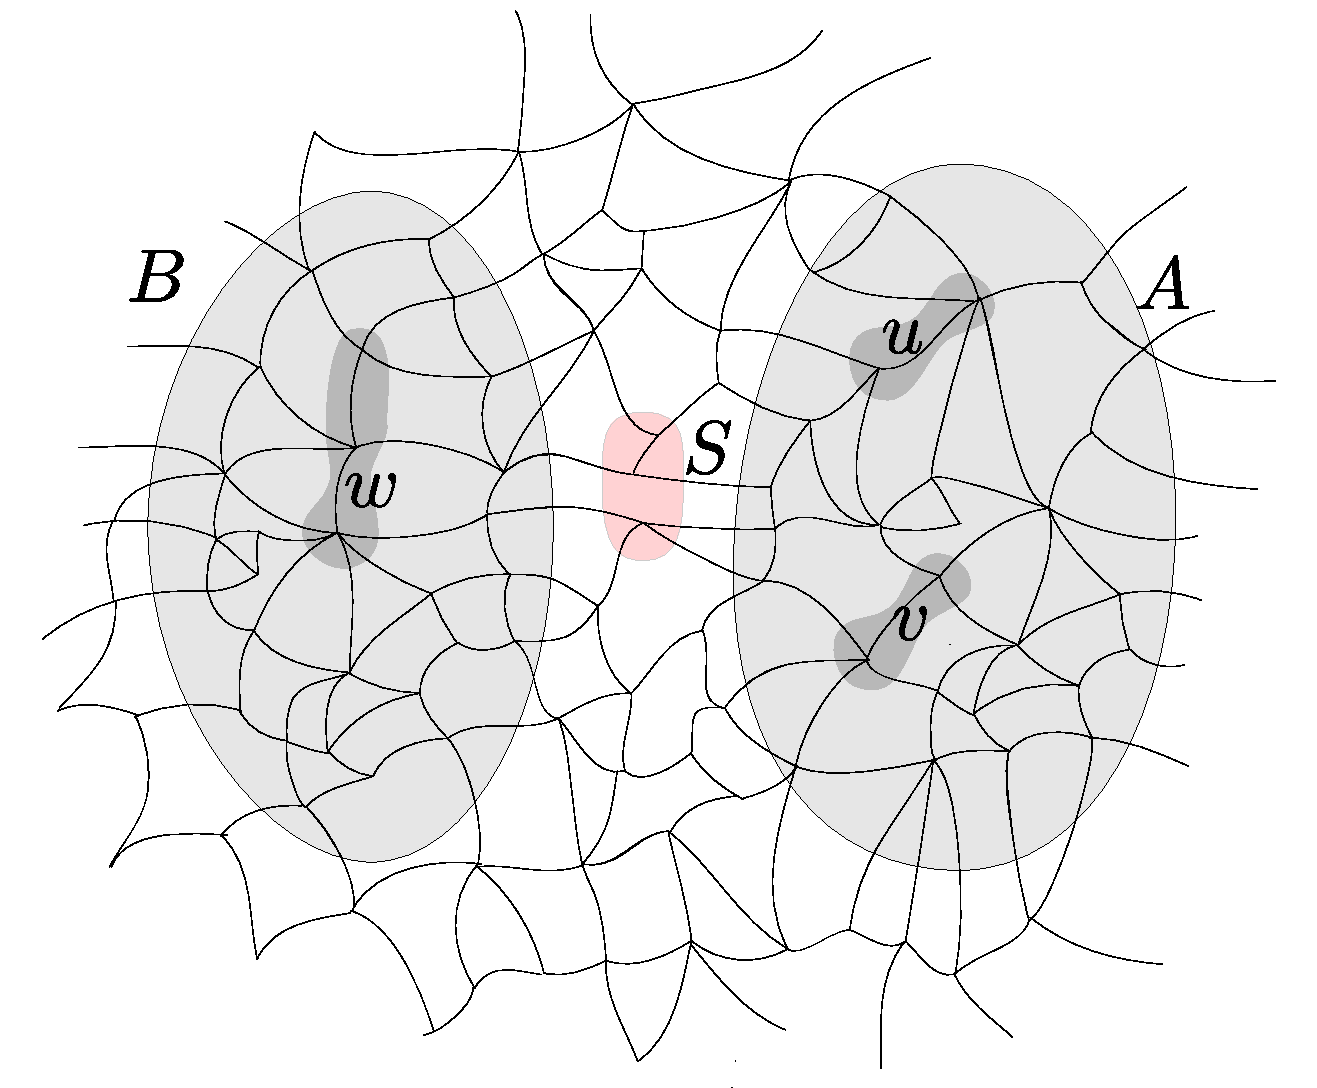
\includegraphics[scale=0.3,page=1]{pics}
% 	\caption{The sets $A$ and $B$ are $2$-separated by $S$.
% 	}
% 	\label{fig:sep}
% \end{figure}
 Observe that taking $r=\infty$ in $r$-separation yields the familiar notion of a separation in graph theory.
From the perspective of stability, separation (for $r=\infty$) characterizes \emph{forking independence} in superflat graphs~\cite{ivanov}. Therefore,
$r$-separation can be thought of as a local analogue of forking independence, for nowhere dense graph classes.

A key lemma concerning $r$-separation (cf. Corollary~\ref{cor:bound}) states that if $A$
and $B$ are $r$-separated by a set $S$ of size $s$ in $G$,
then for any fixed formula $\phi(\bar x,\bar y)$
of quantifier rank $\Oof(\log r)$,
the set  $\{\{\tup v\ \in B^{|\bar y|} : G\models\phi(\tup u,\tup v)\} : \tup u\in A^{|\bar x|}\}$ has cardinality bounded by a constant depending on $s$ and~$\phi$ only (and not on $G,A,$ and $B$). 
This elementary result combines Gaifman's locality of first order logic (cf.~\cite{gaifman1982local}) and a Feferman-Vaught compositionality argument. This, in combination with the polynomial bounds 
for uniform quasi-wideness (Theorem~\ref{thm:new-uqw}, and its extension to tuples~Theorem~\ref{thm:uqw-tuples}), 
as well as the previous results on neighborhood complexity~\cite{drange2016kernelization,eickmeyer2016neighborhood}, are the main ingredients of our main result,~Theorem~\ref{thm:vc-density}.

\paragraph{A duality theorem.}
As an example application of our main result,~Theorem~\ref{thm:vc-density}, we state the following
 result. Below, $\tau(\cal G)$ denotes the \emph{transversality} of $\cal G$, i.e., the least number of elements of a set $X$ which intersects every set in~$\cal G$,
and $\nu(\cal G)$ denotes the \emph{packing number} of $\cal G$, i.e., the largest number of pairwise-disjoint subsets of $\cal G$.
 
%\newcounter{ep}
%\setcounter{ep}{\thetheorem}
\begin{theorem}\label{thm:erdos-posa}
%\begin{restatable}{theorem}{erdosposa}\label{thm:erdos-posa}
	Fix a nowhere dense class of graphs $\CCC$ and a 
	formula $\phi(x,y)$ with two free variables $x,y$.
	Then there is a function $f\from \N\to\N$ with the following property.
	Let $G\in \CCC$ be a graph and let $\cal G$
	be a family of subsets of $V(G)$ consisting of sets of the form $\setof{v\in V(G)}{\phi(u, v)}$, where~$u$ is some vertex of $V(G)$.
Then~$\tau({\cal G})\le f(\nu(\cal G))$.
%\end{restatable}
\end{theorem}

Theorem~\ref{thm:erdos-posa} is an immediate consequence of the bound given by~Theorem~\ref{thm:vc-density} and a result of Matou{\v s}ek~\cite{Matousek:2004:BVI:1005787.1005789}.
%
We remark that a similar, but incomparable result
is proved by Bousquet and Thomass{\'e}~\cite{BousquetT15}.
In their result, the assumption on $\CCC$ is weaker, since they just require that it has \emph{bounded distance VC-dimension}, 
but the assumption on   $\cal G$ is stronger, as it is required to be the set of all balls of a fixed radius.





\paragraph{Stability.}
Finally, we observe that we can apply our  tools to give a constructive proof of the result of Adler and Adler~\cite{adler2014interpreting}
that every nowhere dense class is stable, which yields computable upper bounds on ladder indices.
More precisely, we translate the approach of Podewski and Ziegler~\cite{podewski1978stable} to the finite
and replace the key non-constructive application of compactness with a combinatorial argument based on Gaifman's locality,
in the flavor served by our observations on $r$-separation (Corollary~\ref{cor:bound}).
The following theorem summarizes our result.

% \newcounter{stable}
% \setcounter{stable}{\thetheorem}
%\begin{restatable}{theorem}{newstable}\label{thm:new-stable}
 \begin{theorem}\label{thm:new-stable}
There are computable functions $f\colon \N^3\to\N$ and $g\colon\N\to\N$ with the following property.
Suppose $\phi(\bar x,\bar y)$ is a formula of quantifier rank at most $q$ and with $d$ free variables.
Suppose further that $G$ is a graph excluding $K_t$ as a depth-$g(q)$ minor. Then the ladder index of $\phi(\bar x,\bar y)$ in $G$ is at most $f(q,d,t)$.
 \end{theorem}
%\end{restatable}

%Note that in particular, Theorem~\ref{thm:new-stable} implies that every nowhere dense graph is stable, which was the main conclusion of the paper by Adler and Adler~\cite{adler2014interpreting}. 

%\pagebreak

%\paragraph{Organization.} In \autoref{sec:prelim} we recall some standard concepts from the theory of sparse graphs.
%In~\autoref{sec:uqw} we  prove Theorem~\ref{thm:new-uqw}, improving the previously known bounds and making them constructive. We remark that this result is not needed in the proof of our main result,~Theorem~\ref{thm:vc-density}. The following two sections
% contain the main tools needed in the proof of the main result:
%in~\autoref{sec:uqw-tuples} we formulate and prove the generalization of uniform quasi-wideness to tuples,~Theorem~\ref{thm:uqw-tuples}, and 
%%This result is new in the context of nowhere dense graph classes, and is an important tool for the further results.
%in \autoref{sec:gaifman} we discuss Gaifman locality for first order logic and derive an elementary variant concerning local separators. 
%In \autoref{sec:types} we prove our main result, Theorem~\ref{thm:vc-density}, and the corresponding lower bounds, Theorem~\ref{thm:vc-density-lower-bound}.
%Finally, in \autoref{sec:stable} we provide a constructive proof of the result of Adler and Adler, Theorem~\ref{thm:new-stable}.

\paragraph{Acknowledgments.} We would like to
thank Patrice Ossona de Mendez for pointing us to the
question of studying VC-density of nowhere dense graph
classes.


%\pagebreak
% \todo{page break here?}
